%   Filename    : chapter_4.tex 
\chapter{Preliminary Results/System Prototype}
This chapter presents the preliminary results of the study, including findings from data gathering, the system's diagrams and designs, initial user interface (mockup UI) for the front end, and the chatbot's design.

\section{Data Gathering Results}
The research process for developing TUKIB started with a comprehensive visit to the UPV RRC during the researchers' internship. This phase involved engaging with key personnel and understanding the intricacies of the center's operations. The following sections detail the key activities and information undertaken and gathered during this visit.

\subsection{Facility Tour}
During the researcher's visit, they met with the center's director, administrative staff, and laboratory heads. This introduction provided valuable insights into the roles and responsibilities of various individuals and departments within the UPV RRC. Understanding these dynamics was crucial for tailoring the system to fit the center’s workflows.

The researchers were also given a guided tour, which provided an overview of various laboratories and services offered. These services include:

\begin{itemize}
	\item \textbf{Sample Processing.}The RRC provides sample processing services, essential for research and analysis.
	\item \textbf{Laboratory Equipment Rental} Various pieces of laboratory equipment are available for rent, which supports a wide range of scientific projects.
	\item \textbf{Training and Workshops.} The RRC offers training sessions on laboratory equipment, promoting user proficiency.
	\item \textbf{Facility Rental.} Spaces in the RRC like the Audio-Visual Room (AVR) and conference rooms, ideal for presentations, meetings, and events, are also available for rentals.
\end{itemize}

Each laboratory, including the Biology, Microbiology, Nanotechnology, and Applied Chemistry labs, was introduced in detail, with specific equipment and services discussed in terms of their availability and purpose. The UPV RRC houses five (5) laboratories, namely: Biology, Microbiology, Nanotechnology, Applied Chemistry Laboratory, and Food, Feeds, and Functional Nutrition Laboratory.

\subsection{Stakeholder Identification and Engagement}
The success of workflow automation hinges on understanding the needs and expectations of its key stakeholders. These stakeholders include the RRC laboratory and administrative staff, the clients (university and student researchers and external users of the RRC facilities), the developers, and the member/s of the Computer Science Faculty guiding the project.

The researchers' interaction with the stakeholders allowed the gathering of valuable feedback on the existing system and the challenges that the institution faces. This feedback played a crucial role in shaping the direction of this study's system design, as it highlighted the need for automation, service tracking, and streamlined communication between stakeholders. Additionally, stakeholders were interviewed on their specific needs and pain points. These discussions led to the creation of user stories, which helped to contextualize the requirements from various perspectives. 

This in-depth exposure to the center’s operations was essential for the initial design and development phase of TUKIB, providing a strong foundation for creating a system tailored to the specific needs of the RRC.

\subsection{Scope and Limitations of the Services}
Through direct discussions with the center’s director and administrative staff, the researchers obtained a clear picture of the scope of services provided by each facility, as well as the current limitations they face. Some of these limitations include:

\begin{itemize}
	\item The UPV RRC currently has no website available to the public which describes its mission, vision, services offered, as well as, steps on how to request a service, and other relevant information.   This limits clients from acquiring necessary information about the center and its services. The only platform that they currently utilize for disseminating news, activities, and information about their services is through a Facebook page which lacks structure and organization.
	\item The staff also has difficulty in tracking equipment and facility availability in real-time, as it is essential to ensure that no one else is using an equipment or facility before it can be rented out on a specific time and date.
	\item Manual service request and data management are also a problem as the RRC’s current system relies mainly on Google Forms and Sheets, which poses challenges in efficiency.
\end{itemize}

\subsection{User Requirements}

Based on the gathered data with stakeholders and observations during the facility tour, several key user requirements were identified for the development of TUKIB. 

\begin{itemize}
	\item \textbf{Service Information Accessibility}
	
	A site that allows clients or researchers to gain information about the UPV RRC and what services it provides along with the steps on how to avail those services. 
	
	\item \textbf{Automated Service Requests}
	
	A system that automates service request processes so that staff no longer need to reply to them via email and list the request details manually. 
	
	\item \textbf{Equipment and Facility Availability Tracking}
	
	A system that automates the tracking of the availability of equipment and facilities. This includes a calendar that tracks the facility availability schedule and an equipment inventory management system. 
	
	\item \textbf{Data Management and Reporting}
	
	A system for managing data related to client transactions, service requests, equipment use, and facility bookings. This system should support generating detailed reports for monitoring and decision-making.
	
	\item \textbf{User Account Management}
	
	A system to monitor client profiles and their transaction history with the UPV RRC, including payments, requests, and feedbacks.
	
	\item \textbf{Feedback Mechanism}
	A feedback mechanism that allows clients to complete a service feedback survey and automatically generate feedback statistics for easier feedback analysis.
	
\end{itemize}

\section{System Design}

\subsection{Process Flow Diagram}

\figref{fig:process_flow} illustrates the complete service delivery process of the UPV RRC through TUKIB. The process begins with a service request from the client and proceeds through multiple stages, including review and approval, and execution of the service. The process concludes with collecting a feedback from the client, providing opportunities for continuous improvement.

\begin{figure}[h]
	\centering 
	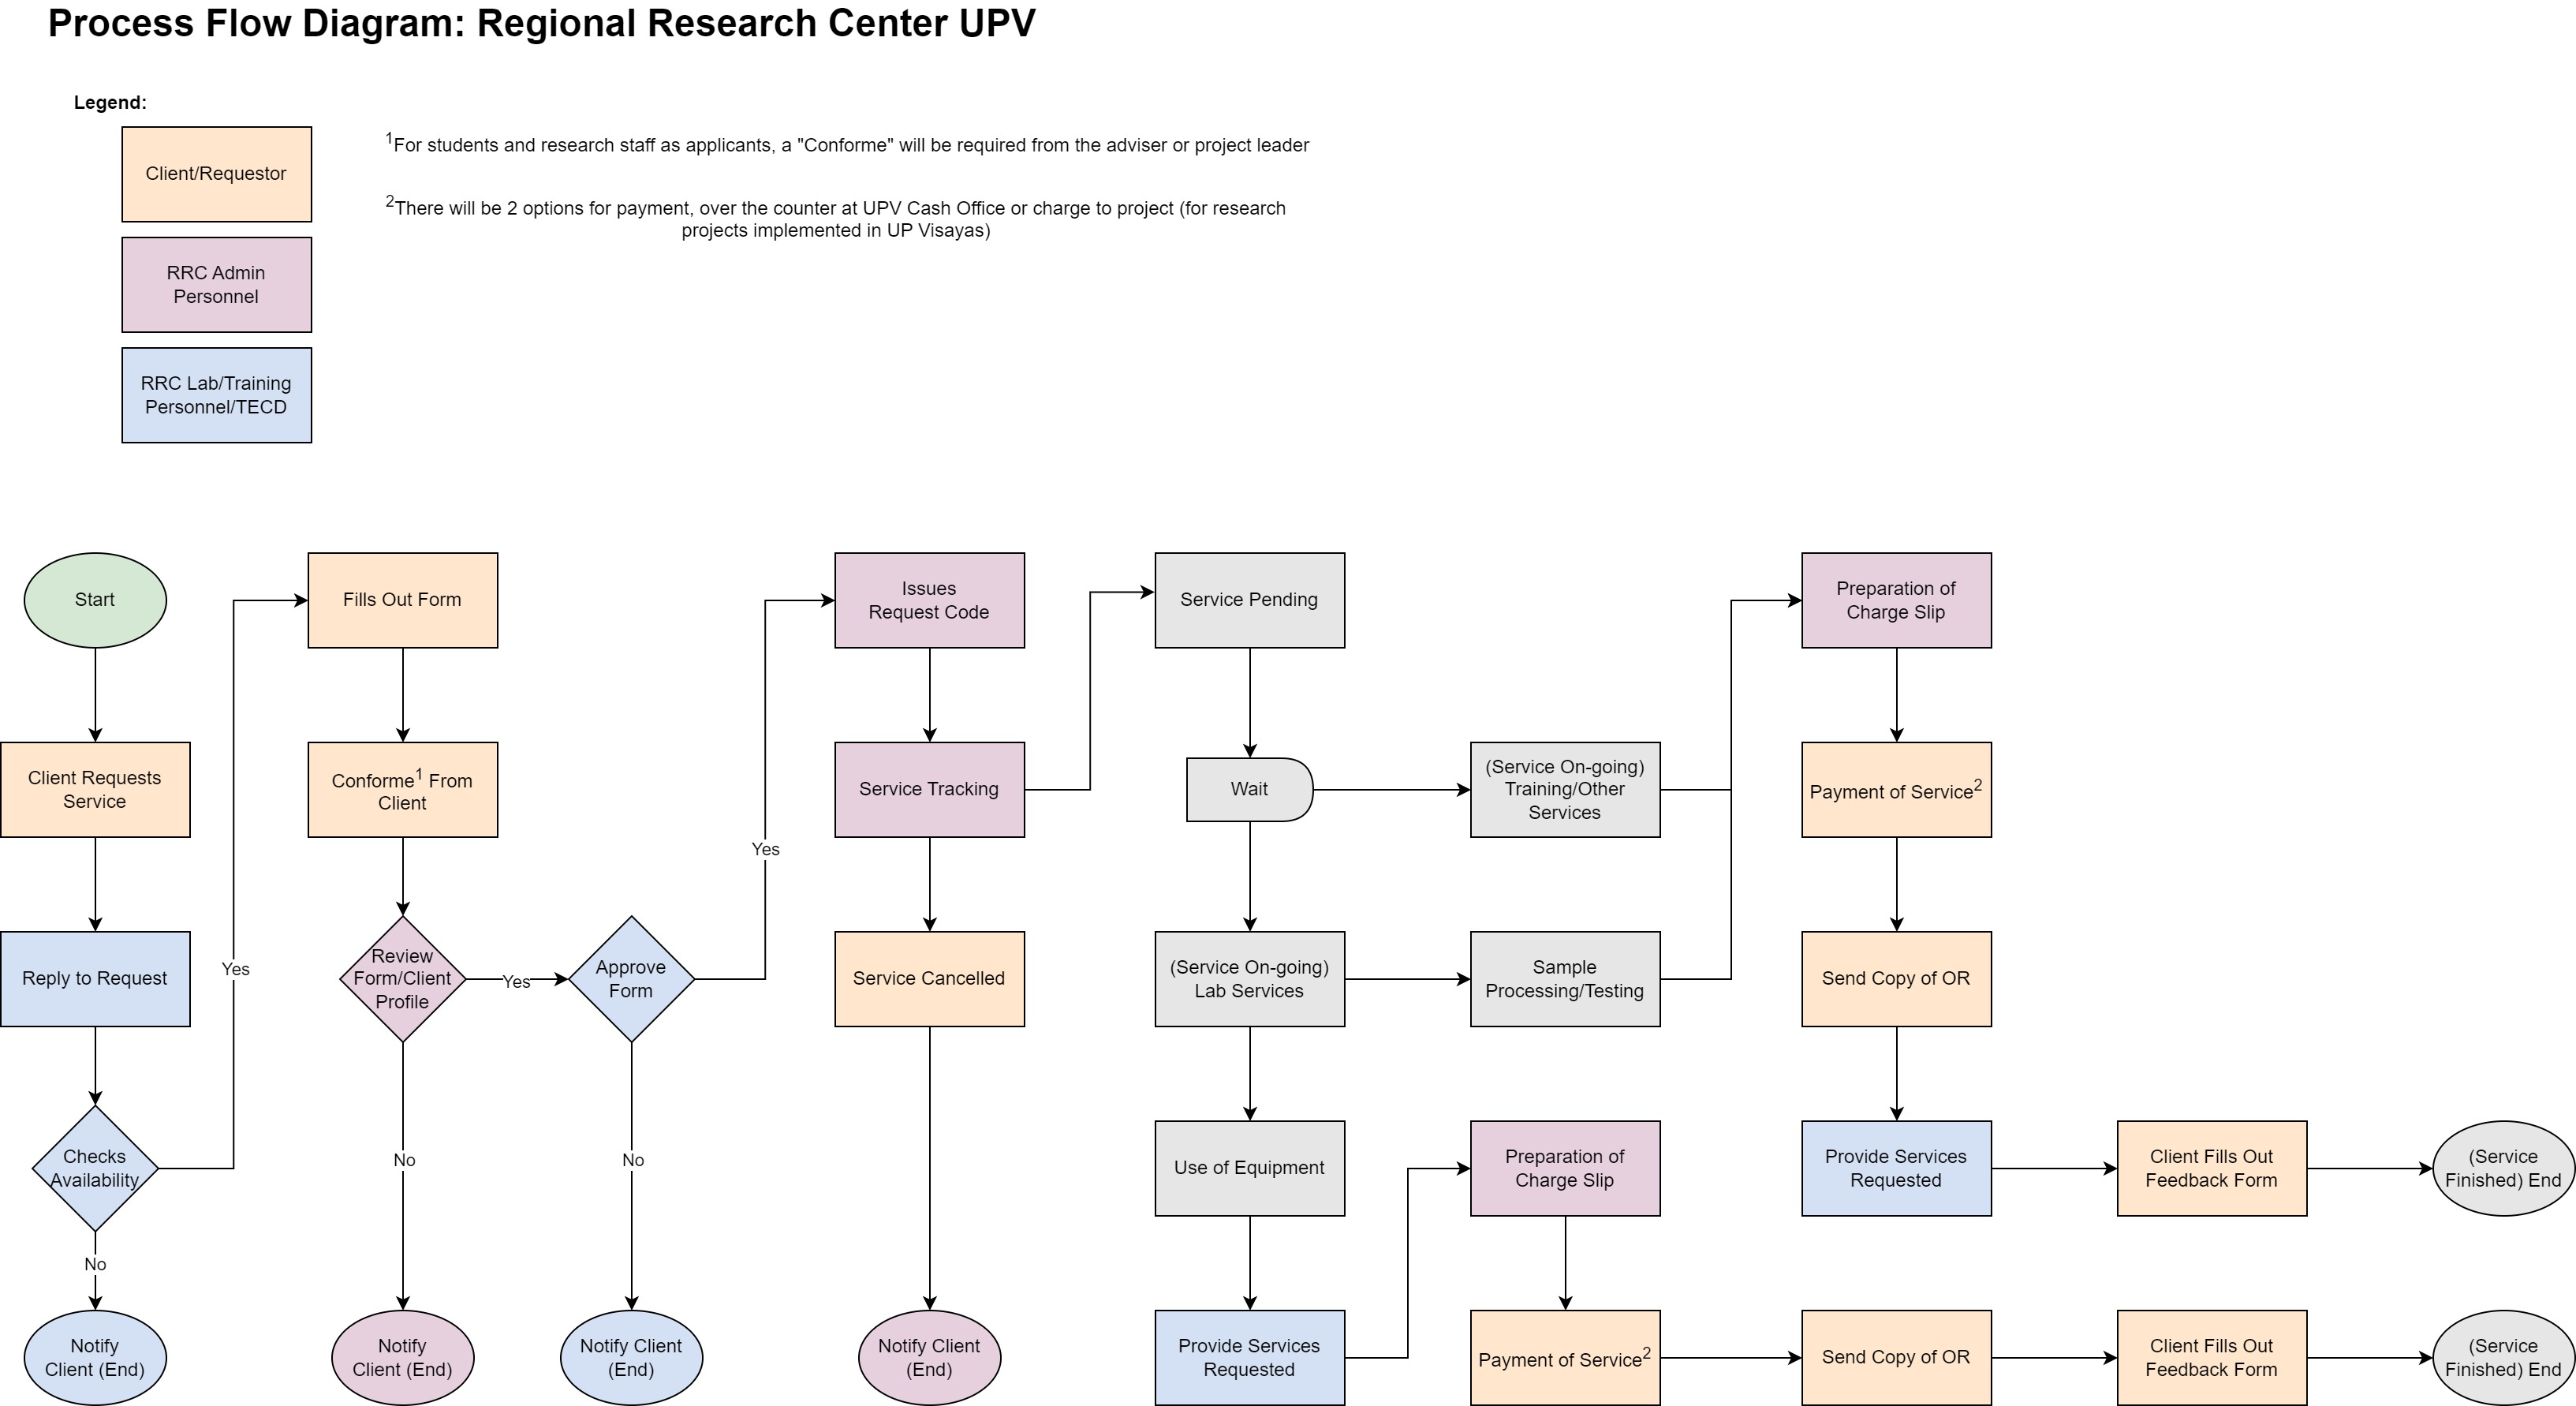
\includegraphics[width=1\textwidth]{process_flow.jpg}
	\caption{Process Flow Diagram}
	\label{fig:process_flow}
\end{figure}

\newpage

\subsection{Context Model}

\figref{fig:context_model} illustrates the interactions between the system and both internal and external entities. It shows how the system communicates with different stakeholders, including client, staff, director, and university researcher. The model also outlines how information flows from entities to the system and vice versa, showing how it works and its role within the institution.

\textbf{Clients} will primarily interact with the system to make service inquiries or submit requests related to the services offered by the UPV RRC. They might also provide feedback or report issues based on their interactions with the system or their overall experience on transacting with the UPV RRC.

For the \textbf{University Researchers}, they can use the system to oversee any laboratory-related requests, such as assessing, approving and terminating requests. Additionally, they can also use the system to release the results of the service rendered, if the client wishes to have it in softcopy. 

Similarly, \textbf{TECD Staff} can use the system to oversee, equipment or facility rental related requests. This also includes assessing, approving, and terminating request. 

For the \textbf{Admin Staff}, the system will provide oversight on the ongoing transactions. Admin staff ensure that users from various roles perform their duties effectively by managing accounts, permissions, and system-wide configurations. Like the university researchers and TECD staff, they also have access on the service-related requests and have an ability to assess, approve, and terminate transactions or requests.

Moreover, the system will provide full oversight of activities to the \textbf{Director}, offering comprehensive visibility and control. Furthermore, the Director will have access to detailed statistics and insights about the services offered, enabling the institution to make informed and strategic decisions.

\begin{figure}[h]
	\centering 
	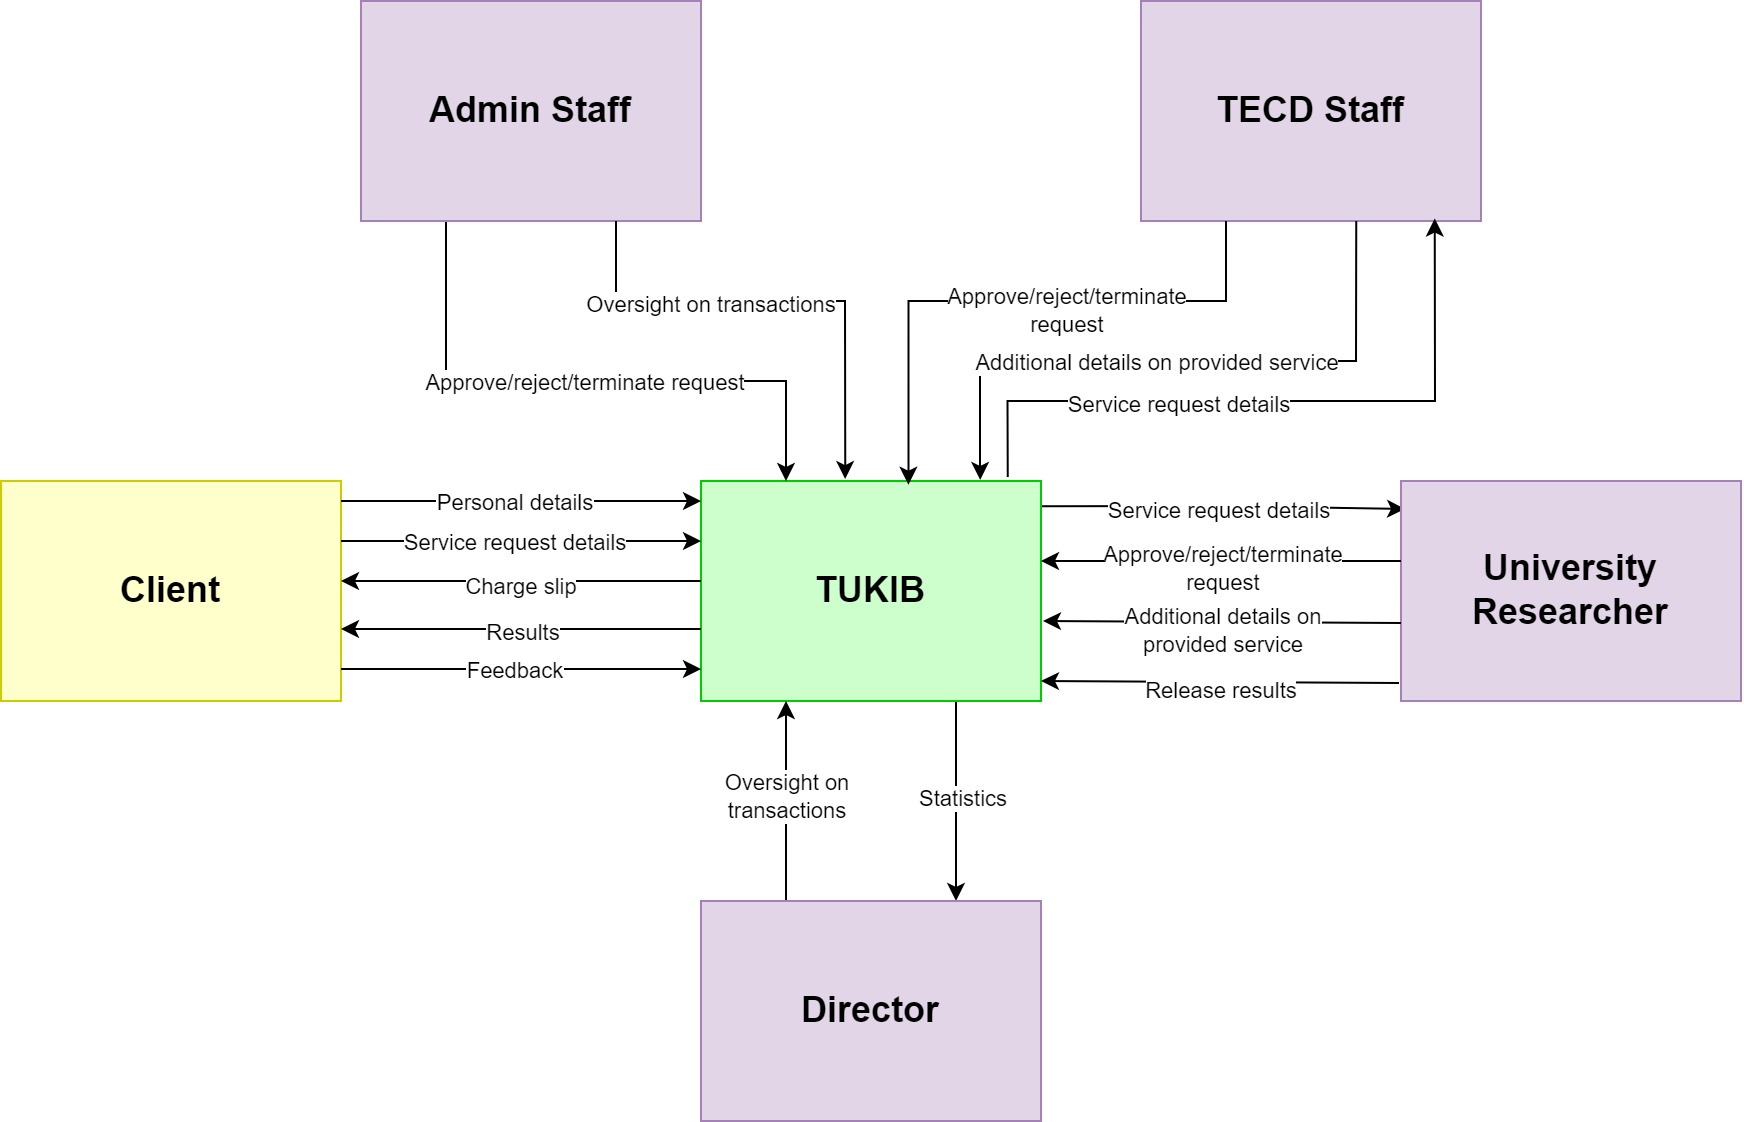
\includegraphics[width=1\textwidth]{context model.png}
	\caption{Context Model}
	\label{fig:context_model}
\end{figure}

\newpage

\subsection{Use Case Diagram}

Figures \ref{fig:use_case_client}, \ref{fig:use_case_admin}, \ref{fig:use_case_director}, and \ref{fig:use_case_staff} present the use case diagrams of the system, which visually represent the key interactions between different types of users and the system in the service management cycle of the UPV RRC. The diagrams highlight the various roles and their associated tasks in managing service requests.

\newpage

\begin{figure}[h]
	\centering
	\begin{minipage}{0.30\textwidth}
		\centering
		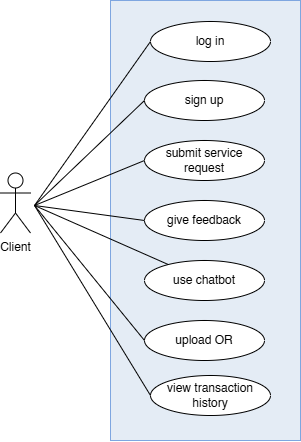
\includegraphics[width=\textwidth]{use_case_client.jpg}
		\caption{Use Case Diagram (Client interface)}
		\label{fig:use_case_client}
	\end{minipage}%
	\hfill
	\begin{minipage}{0.32\textwidth}
		\centering
		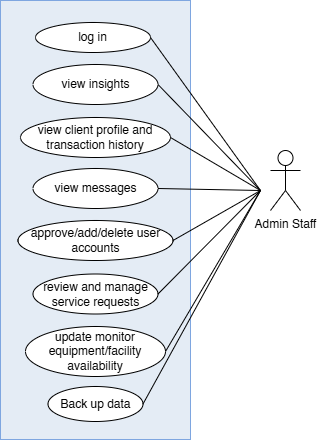
\includegraphics[width=\textwidth]{use_case_admin.jpg}
		\caption{Use Case Diagram (Admin interface)}
		\label{fig:use_case_admin}
	\end{minipage}
	
	\vspace{0.5cm} % Add some vertical space between the rows
	
	\begin{minipage}{0.30\textwidth}
		\centering
		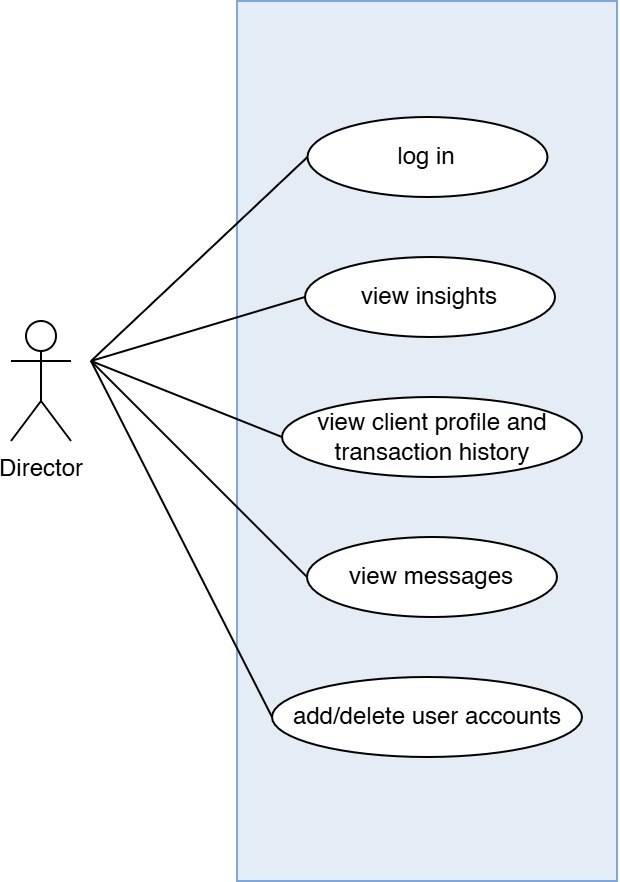
\includegraphics[width=\textwidth]{use_case_director.jpg}
		\caption{Use Case Diagram (Director interface)}
		\label{fig:use_case_director}
	\end{minipage}%
	\hfill
	\begin{minipage}{0.30\textwidth}
		\centering
		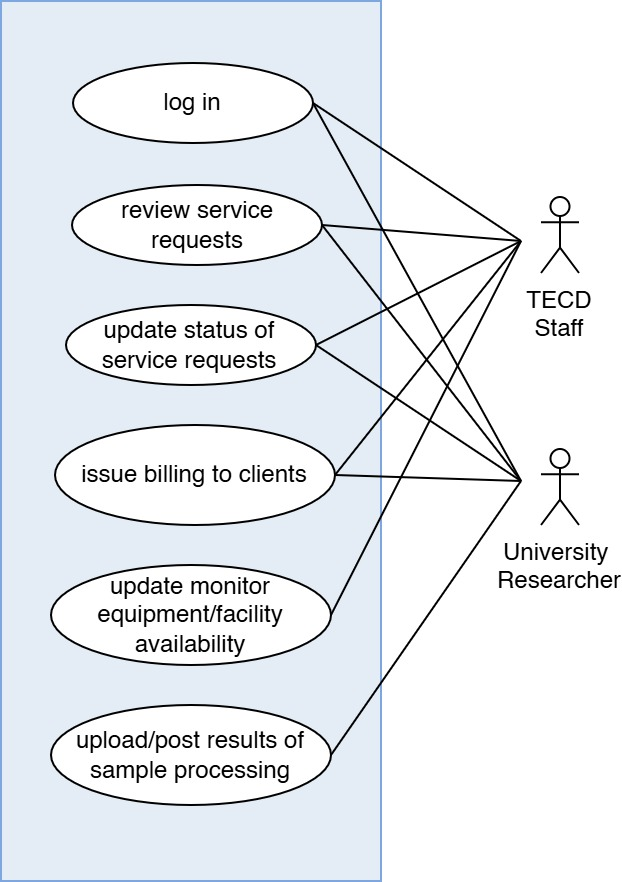
\includegraphics[width=\textwidth]{use_case_staff.jpg}
		\caption{Use Case Diagram (TECD and UR interface)}
		\label{fig:use_case_staff}
	\end{minipage}
\end{figure}

\newpage

\subsection{Data Flow Diagram}

\figref{fig:data_flow} shows the flow of data within the system, illustrating how information is exchanged between different components and users through the entire service request and delivery process of the UPV RRC. The diagram also illustrates the pathways through which data moves, providing overview into how information are stored and retrieved within the system.

\begin{figure}[h]
	\centering 
	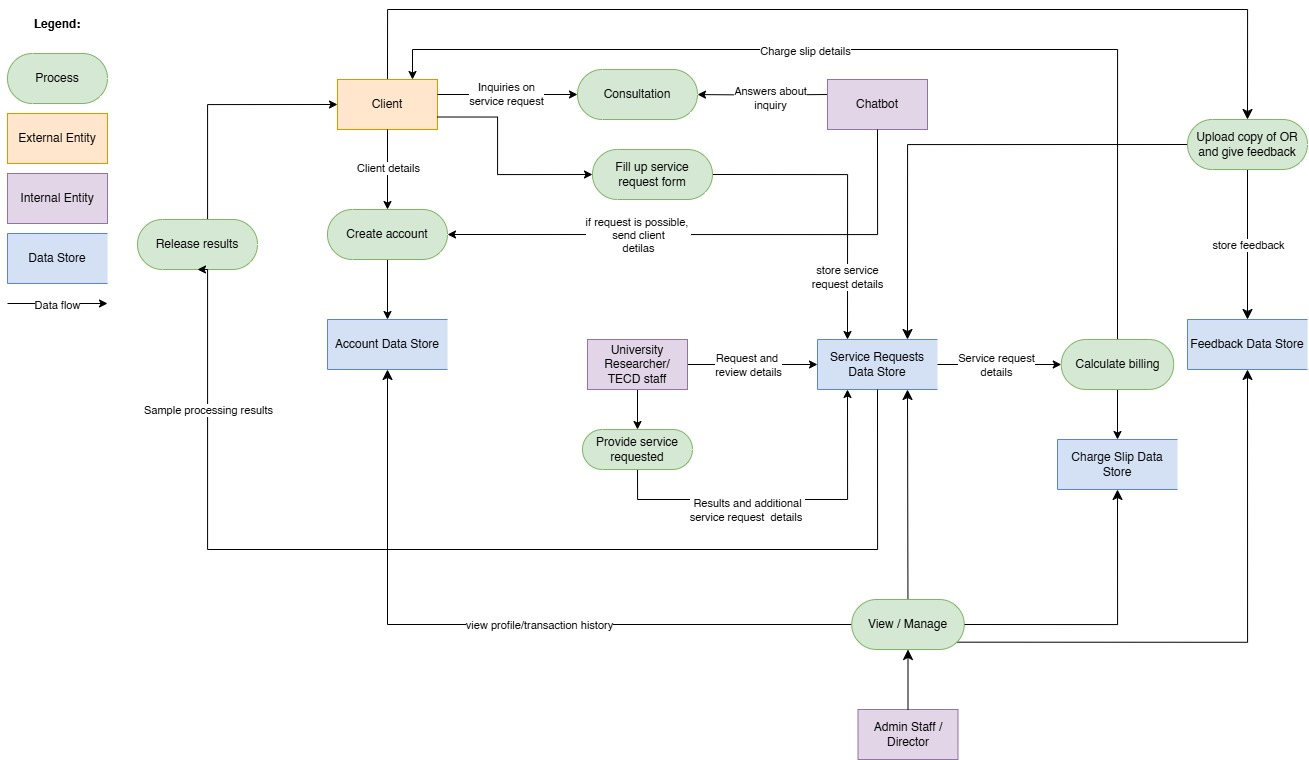
\includegraphics[width=1\textwidth]{data_flow.jpg}
	\caption{Data Flow Diagram}
	\label{fig:data_flow}
\end{figure}

\subsection{Database Diagram}

The database design for TUKIB revolves around tracking and managing various service related data through several interrelated entities to ensure easy storing and retrieval. As seen in \figref{fig:database}, there are a total of 11 tables in the database design for the TUKIB. 

The \textbf{client} table stores essential information about the clients, such as their name, contact details, and addresses. Similarly, the \textbf{staff} table also stores the necessary details of staff including name, contact details, and position. 

When a client wishes to avail a service, a corresponding \textbf{service request} is created, linking the request to both the client and the staff members handling the service. This table also records the type of service (e.g., use of equipment, use of facility, sample processing, or training) and its status. To track the usage of specific resources, there are separate tables for the \textbf{use of equipment} and \textbf{use of facility}, which log the details of which equipment or facility was used for a particular service request, including the time of use and duration. For other services, the \textbf{sample processing} table tracks the handling and status of samples, while the \textbf{training service} table records information about any training sessions provided to clients, including the assigned staff and training details. The \textbf{equipment} table stores the information about availability of equipments and history usage. 

Once the requested service is rendered, the \textbf{charge slip} table handles the relevant information needed for billing including the cost of the service. Consequently, the \textbf{payment} table ensures that all transactions are logged, tracking the payment amounts and methods linked to specific services. Additionally, feedback from clients on their experience on availing a service is stored in the \textbf{feedback} table, providing valuable insights into the service quality and client satisfaction.

\begin{figure}[h]
	\centering 
	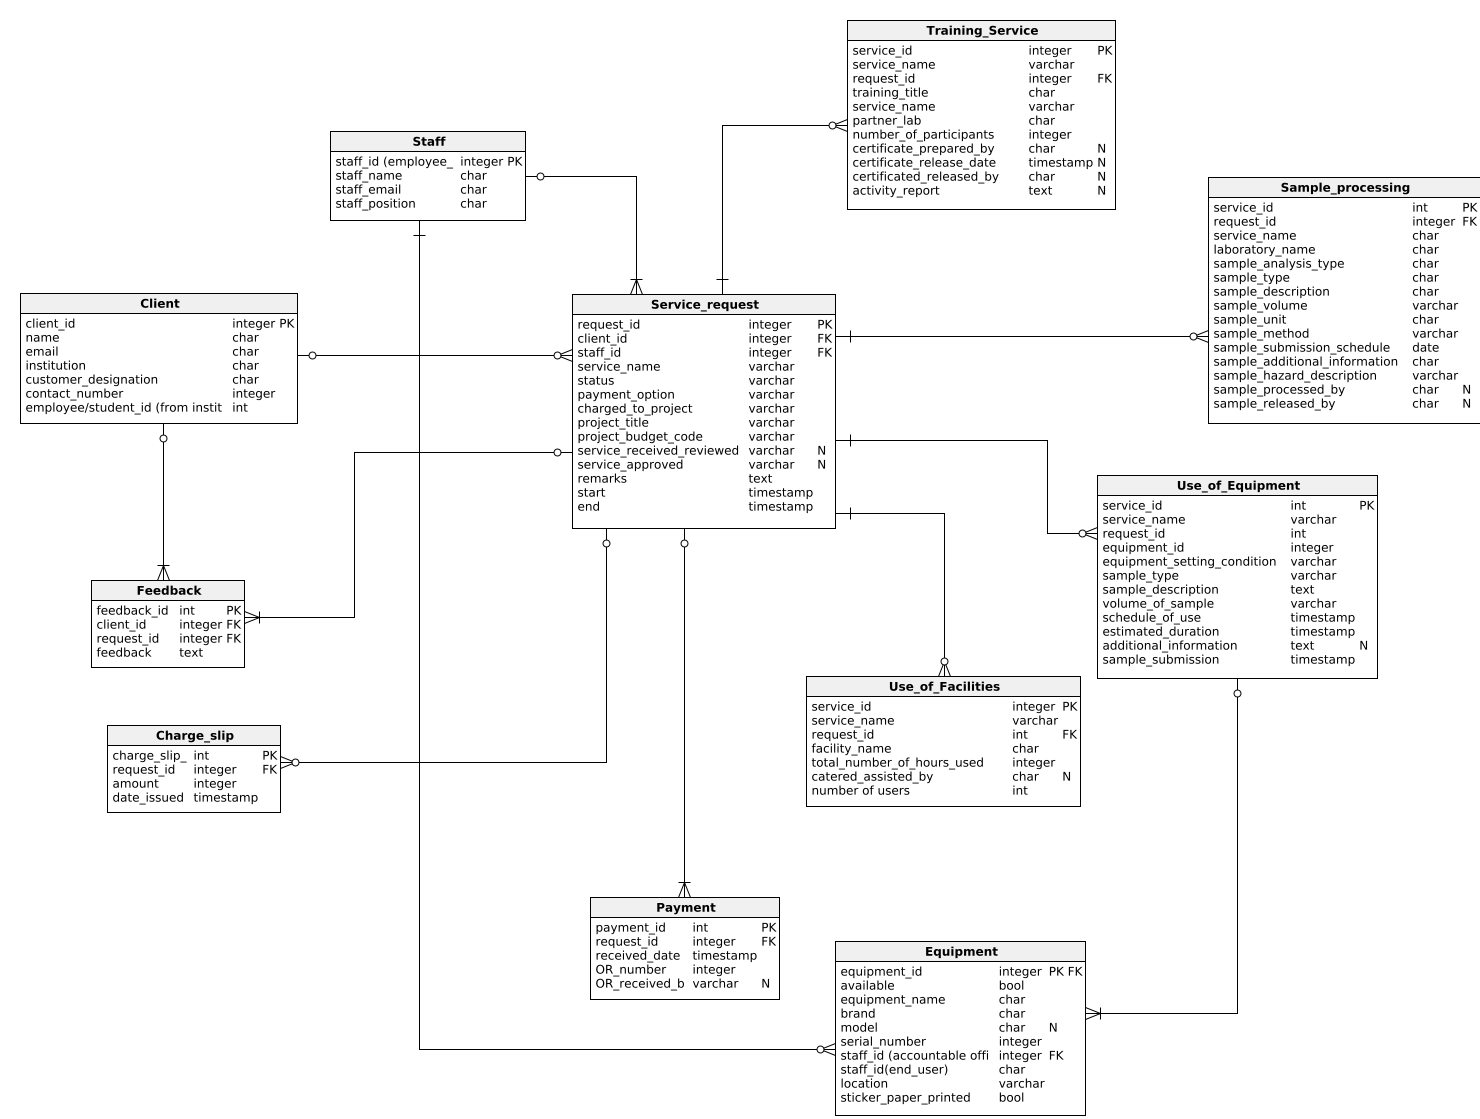
\includegraphics[width=1\textwidth]{database.png}
	\caption{Database Design Diagram}
	\label{fig:database}
\end{figure}

\newpage

\section{Chatbot}

\textbf{Entities and Intents}

From the data gathering phase, the developers were able to identify common user queries and specific service requirements needed for the development of the chatbot. The collected data was used to construct the intents and entities which are essential for the chatbot’s functionality. 

Intents represent the goal the users want to achieve when interacting with the chatbot (e.g., ”start consultation,” ”ask about lab rental procedures,” ”inquire about service status”). The intents are divided into greeting, general, service requests, frequently asked questions, feedback, and end or closing message. On the other hand, entities are specific pieces of information that the chatbot needs to get from the user in order to fulfill a task. For example, the chatbot needs to know the name of the equipment and desired time for renting in order to indicate the equipment's availability. 

\newpage

\noindent \textbf{Conversation Flow}

\figref{fig:chatbot_flow} illustrates the conversation flow for TUKIB's chatbot, named LIRA— short for Learning, Innovation, and Research Assistant. LIRA will be accessible throughout the entire website, ensuring that all users, whether logged in or not, can obtain support whenever needed. Users can initiate a chat with LIRA via a persistent button that remains visible across the site or by selecting the dedicated “New Service” button found on the user dashboard.

\begin{figure}[h]
	\centering 
	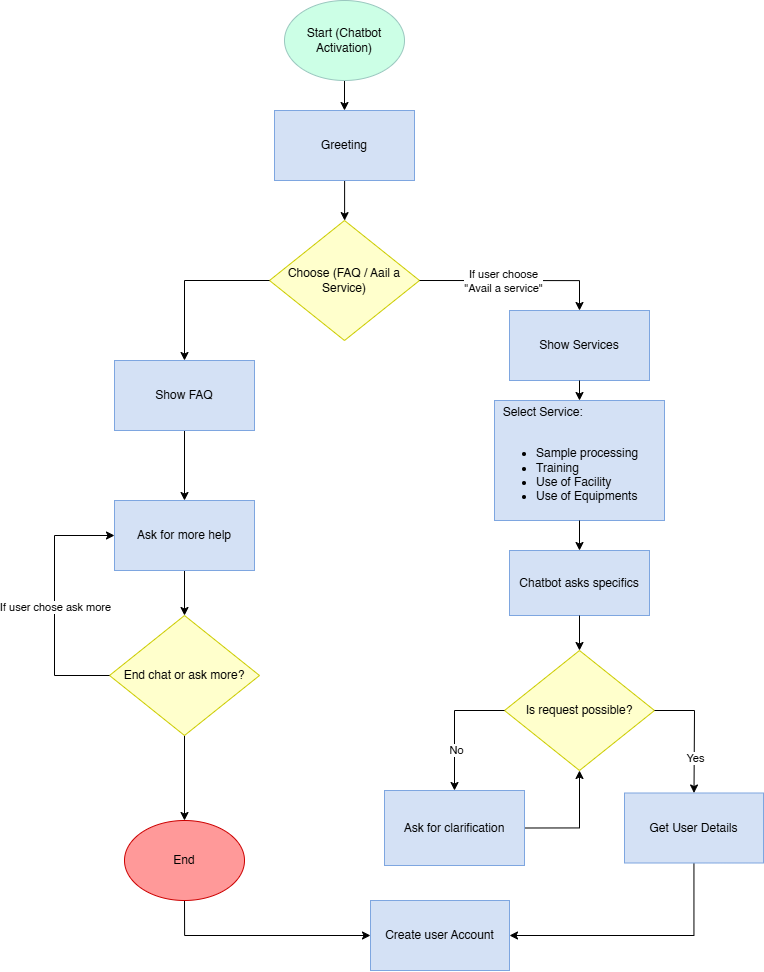
\includegraphics[width=0.7\textwidth]{chatbot_flow.png}
	\caption{LIRA Conversation Flow}
	\label{fig:chatbot_flow}
\end{figure}

\newpage

The structure of the chatbot is centered around a conversational flow that guides users through various tasks, from inquiries to service request consultations. The chatbot’s design consists of the following core components:

\begin{itemize}
	\item \textbf{Welcome Greeting}
	
	Present a welcome message where the chatbot greets users with a friendly introduction and offers assistance, presenting options such as “Service Inquiry“ and “Frequently Asked Questions/FAQs” \newline
	
	\item \textbf{Flow for Service Inquiry}
	
	If the user chooses the option “Service Inquiry,” the chatbot will ask a follow-up question to identify which service the user wishes to inquire about. Sample service choices include sample processing,  lab equipment rental, etc. Then, the chatbot uses the user's answer details to present accurate information about each service. \newline
	
	\item \textbf{Flow for Consultation}
	
	The flow for consultation is designed to facilitate user inquiries about the services they wish to avail. As the primary purpose of the chatbot, this interaction allows users to ask questions about the services offered by RRC. When a user expresses interest, the chatbot engages by asking for specific details related to their request. For instance, if a user inquires about sample processing (e.g., the type of sample and processing methods needed), the chatbot will guide them through the details. This interactive process ensures that users receive tailored information while the chatbot gathers necessary details to asses service feasibility. \newline
	
	\item \textbf{Flow for General Questions / FAQ}
	
	The chatbot should be able to answer and handle frequently asked questions by clients. These would include questions about general services, rental pricing methods, facility rental processes, etc. \newline
	
	\item \textbf{Chatbot User Feedback}
	
	Once the conversation with the chatbot is completed, it will prompt the user to rate or provide feedback on their experience, which will help the developers and the UPV RRC to in enhancing the bot and the customer satisfaction. \newline
	
	\item \textbf{Error Handling}
	
	Chatbot failures will lead to conversational dead ends if not dealt with properly. Thus, negating the main purpose of chatbot in this system which is to provide efficient customer service. To address this, the chatbot will have a fallback mechanism whenever an input from user was unexpected or a system error occurs. For example, if the chatbot cannot understand the user input, there will be rules on how the chatbot would handle this situation. Sample fallback methods would be redirecting the conversation to a live agent. Another option would be presenting friendly-toned error messages to the users, letting them know that the chatbot is having trouble understanding their input.
	 
	\subitem Sample error messages include “Sorry, I didn't catch that. Could you rephrase your question?” or “I'm sorry, I have a hard time understanding. Could you please rephrase your query?” and “I'm sorry, but what you're asking is not clear to me. Could you paraphrase it?”
	
\end{itemize}


\section{System Development}

\subsection{Front-end}

\noindent\textbf{Landing page}

\noindent \figref{fig:landing} showcases the landing page of the website for the system. The page features easy navigation to essential information and pages including home, news, services, contact, and about. A log in button is also included on the top right of the page to ensure that user's can quickly access their accounts. Additionally, the persistent button for the chatbot can be found on the bottom left of the page.

\newpage

\begin{figure}[h]
	\centering 
	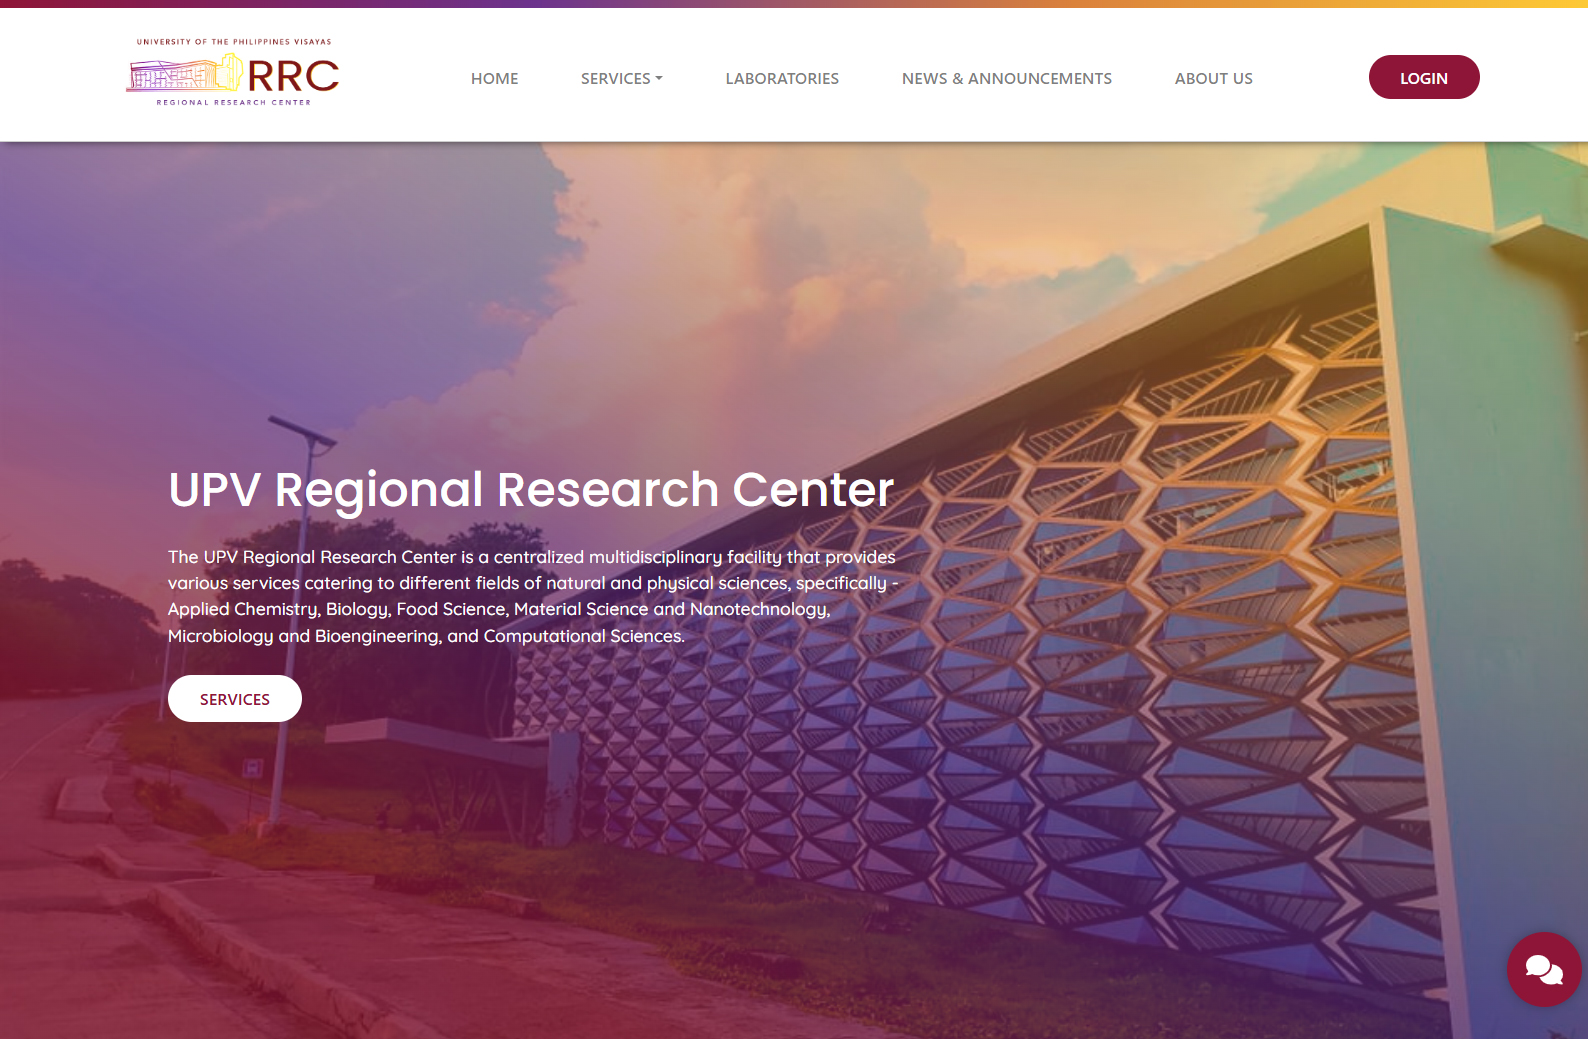
\includegraphics[width=0.8\textwidth]{landing.png}
	\caption{Landing/Homepage}
	\label{fig:landing}
\end{figure}

\noindent \textbf{User authentication}

\noindent All types of users will have pre-made accounts. Staff members will automatically have accounts, while clients will only have accounts created after their first consultation is approved. On the login page, users will need to enter their email address and password. Additionally, Google authentication is available, allowing users to sign in using their Google account for a quicker and more secure login experience. Passwords will be hidden by default, but users can click the eye icon in the password field (as shown in \figref{fig:login}) to toggle visibility. After successfully logging in, users will be redirected to their respective dashboards.

\newpage

\begin{figure}[h]
	\centering
	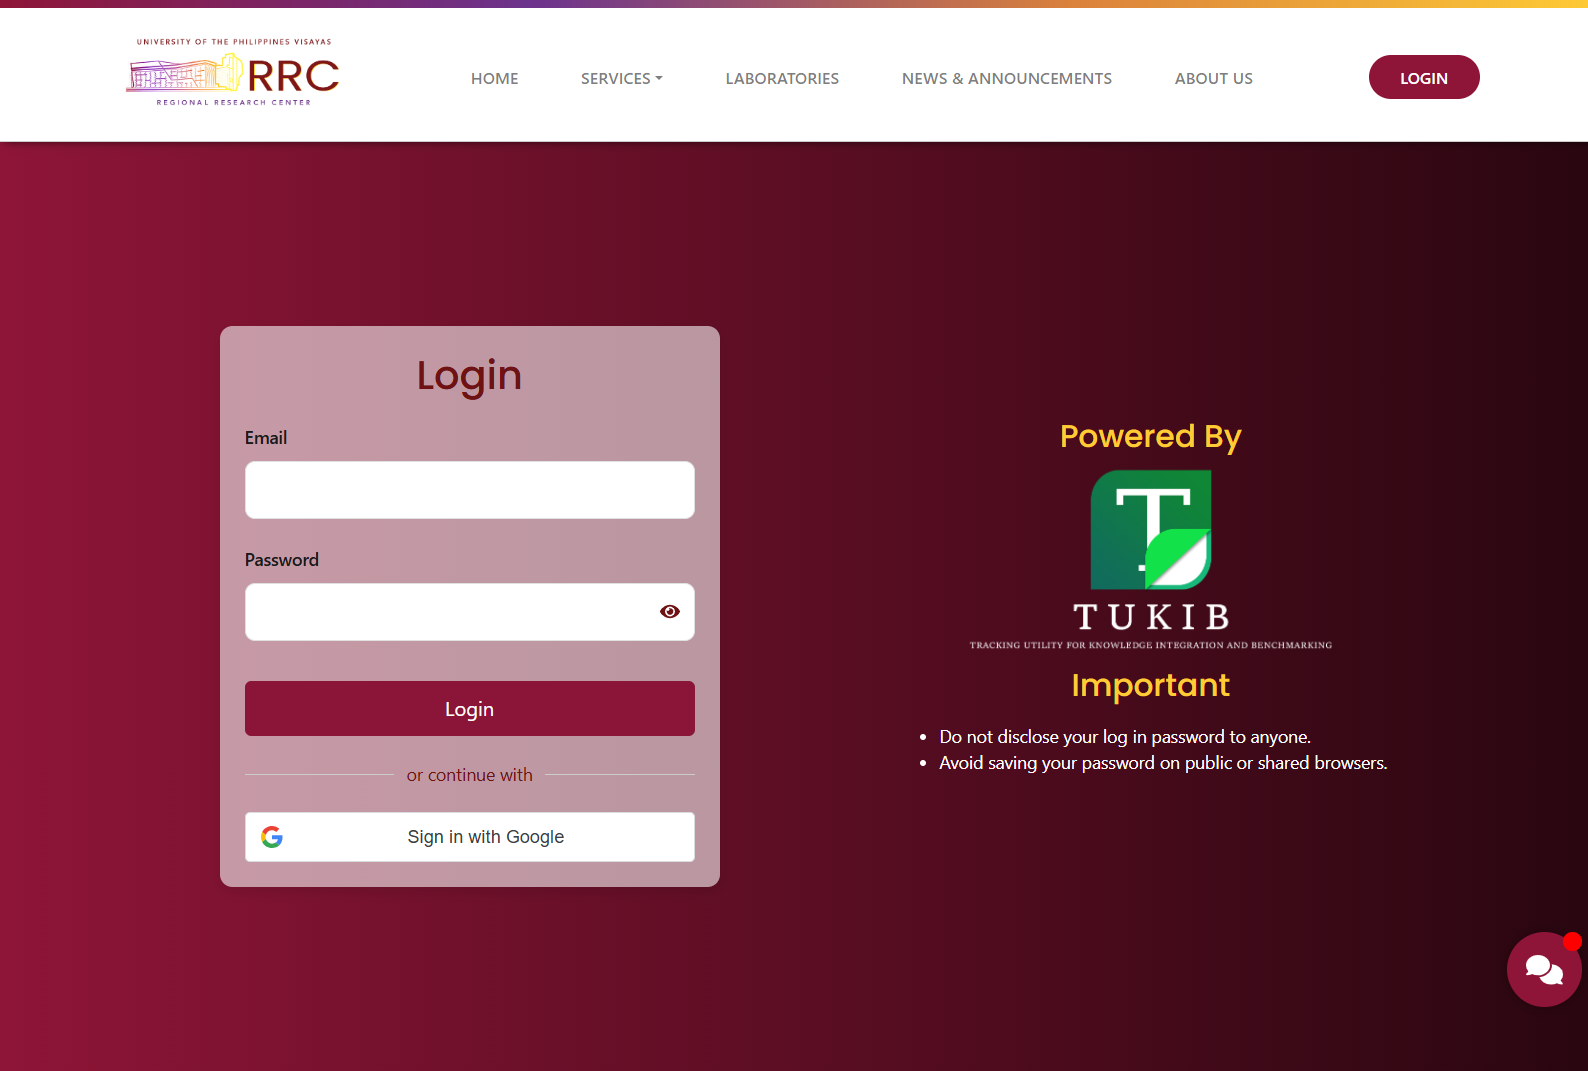
\includegraphics[width=0.80\textwidth]{login.png}
	\caption{Log in page}
	\label{fig:login}
\end{figure}

\begin{figure}[h]
	\centering
	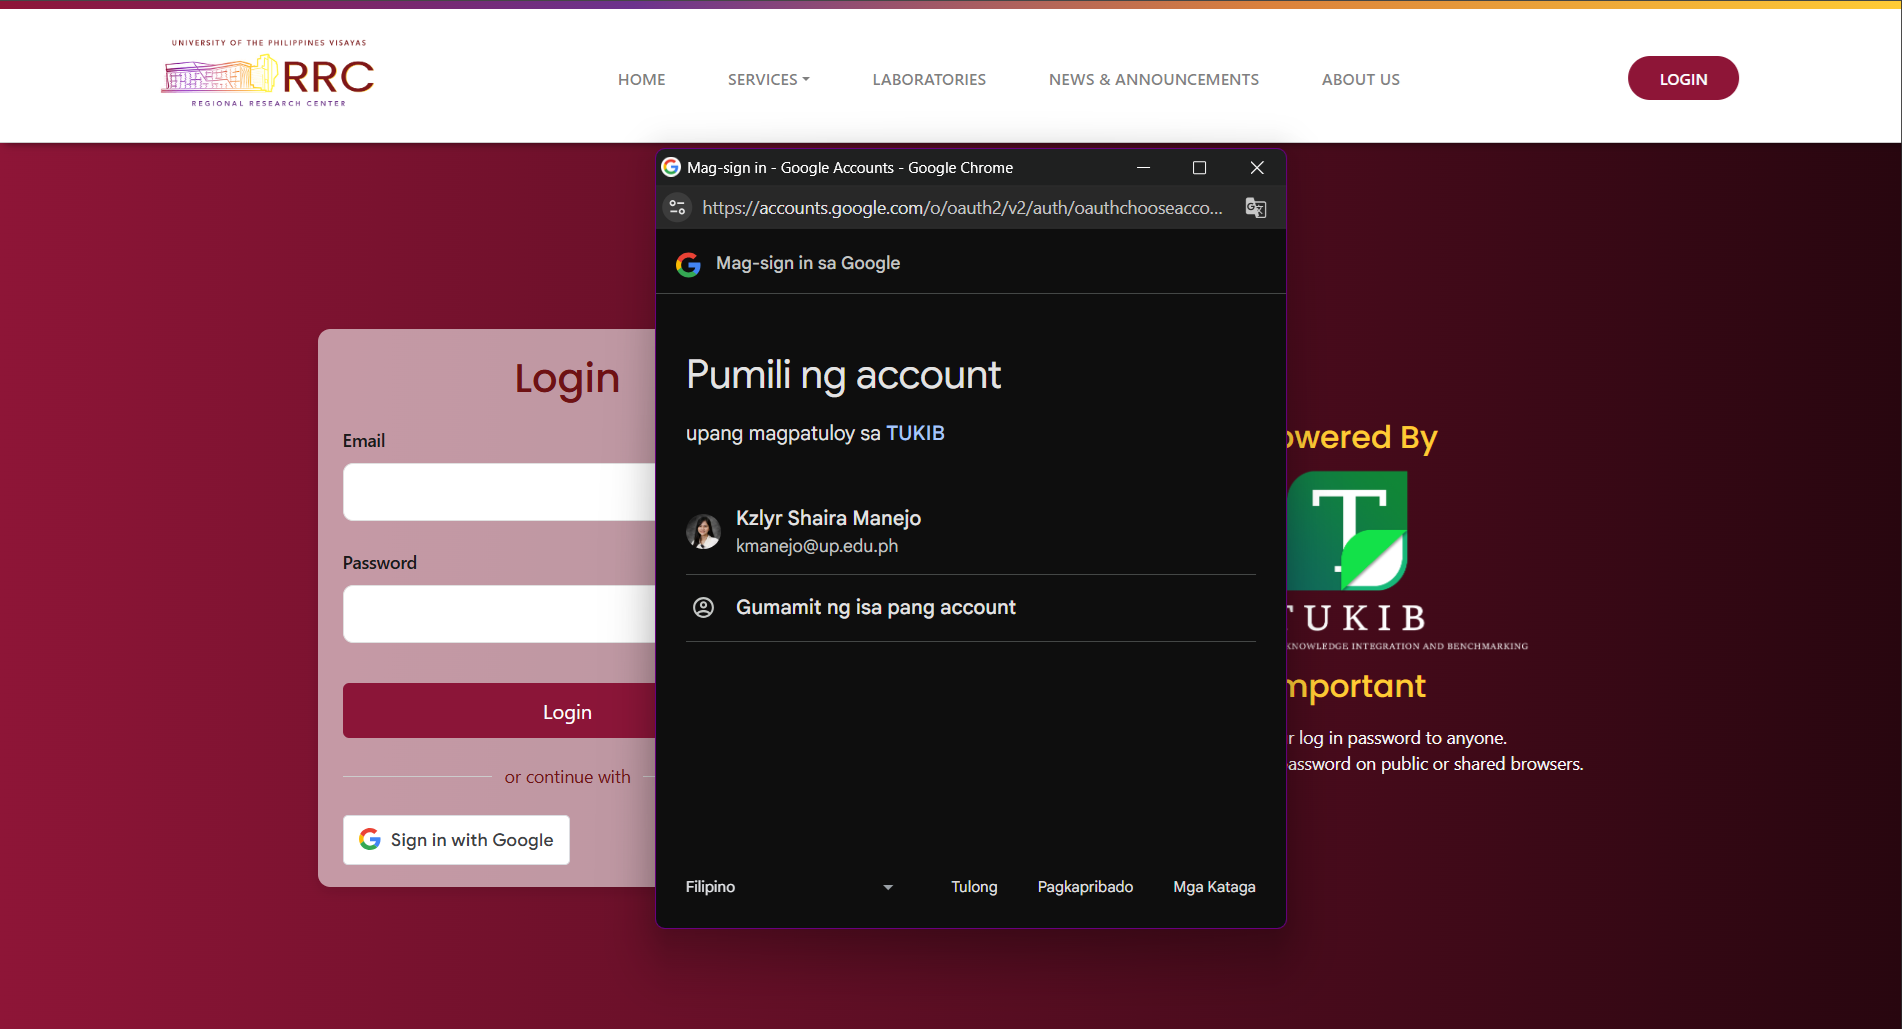
\includegraphics[width=0.80\textwidth]{login_googlesso.png}
	\caption{Log in with Google SSO}
	\label{fig:login_google}
\end{figure}

\noindent \textbf{User Dashboards}

User dashboard is designed for the needs of two primary user groups of TUKIB who are the staff and clients. Each user group has a different user interface to cater to their specific needs as seen from \figref{fig:staff_dashboard} and \figref{fig:client_dashboard}. 

For the client’s user interface, the developers designed a dashboard that shows the user’s profile, transaction history, and a button to avail a new service. For the staffs’ user interface, a layout was designed specifically for their tasks, featuring information and capabilities necessary for efficient management and oversight. This includes tools for monitoring workflows, accessing reports, and managing user requests.

\begin{figure}[h]
	\centering 
	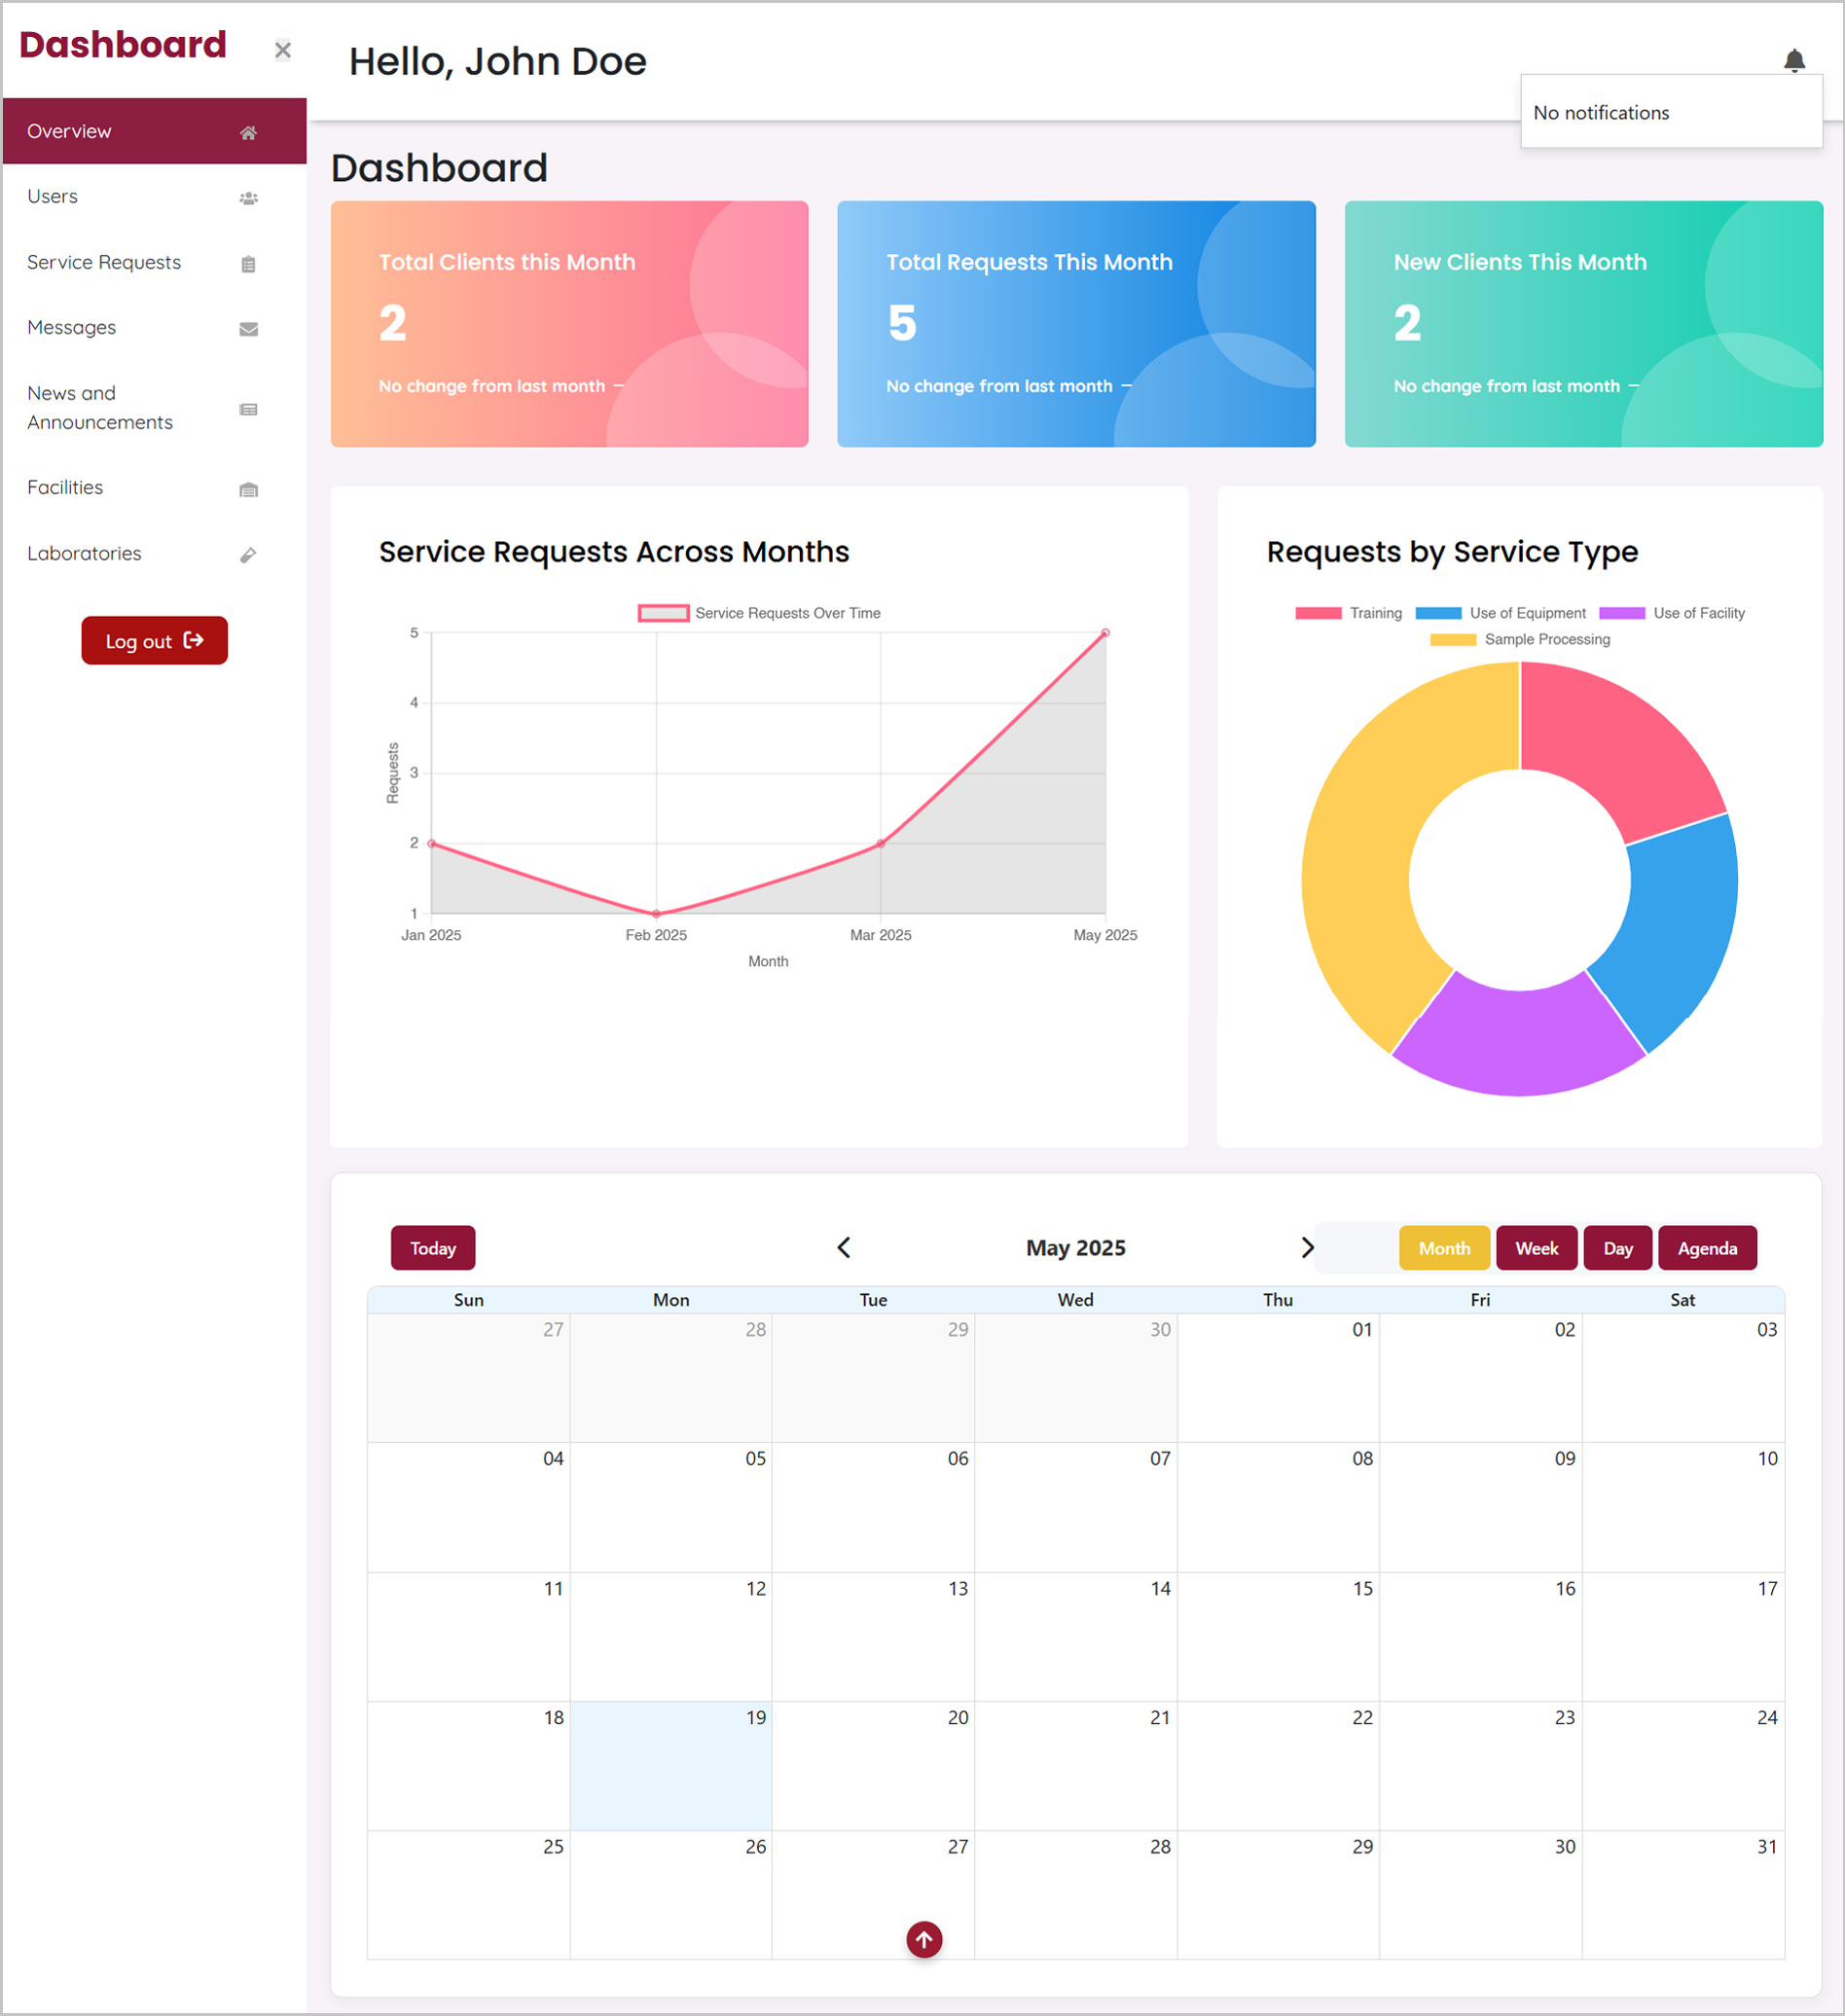
\includegraphics[width=0.8\textwidth]{staff_dashboard.png}
	\caption{Staff dashboard}
	\label{fig:staff_dashboard}
\end{figure}

\begin{figure}[h]
	\centering 
	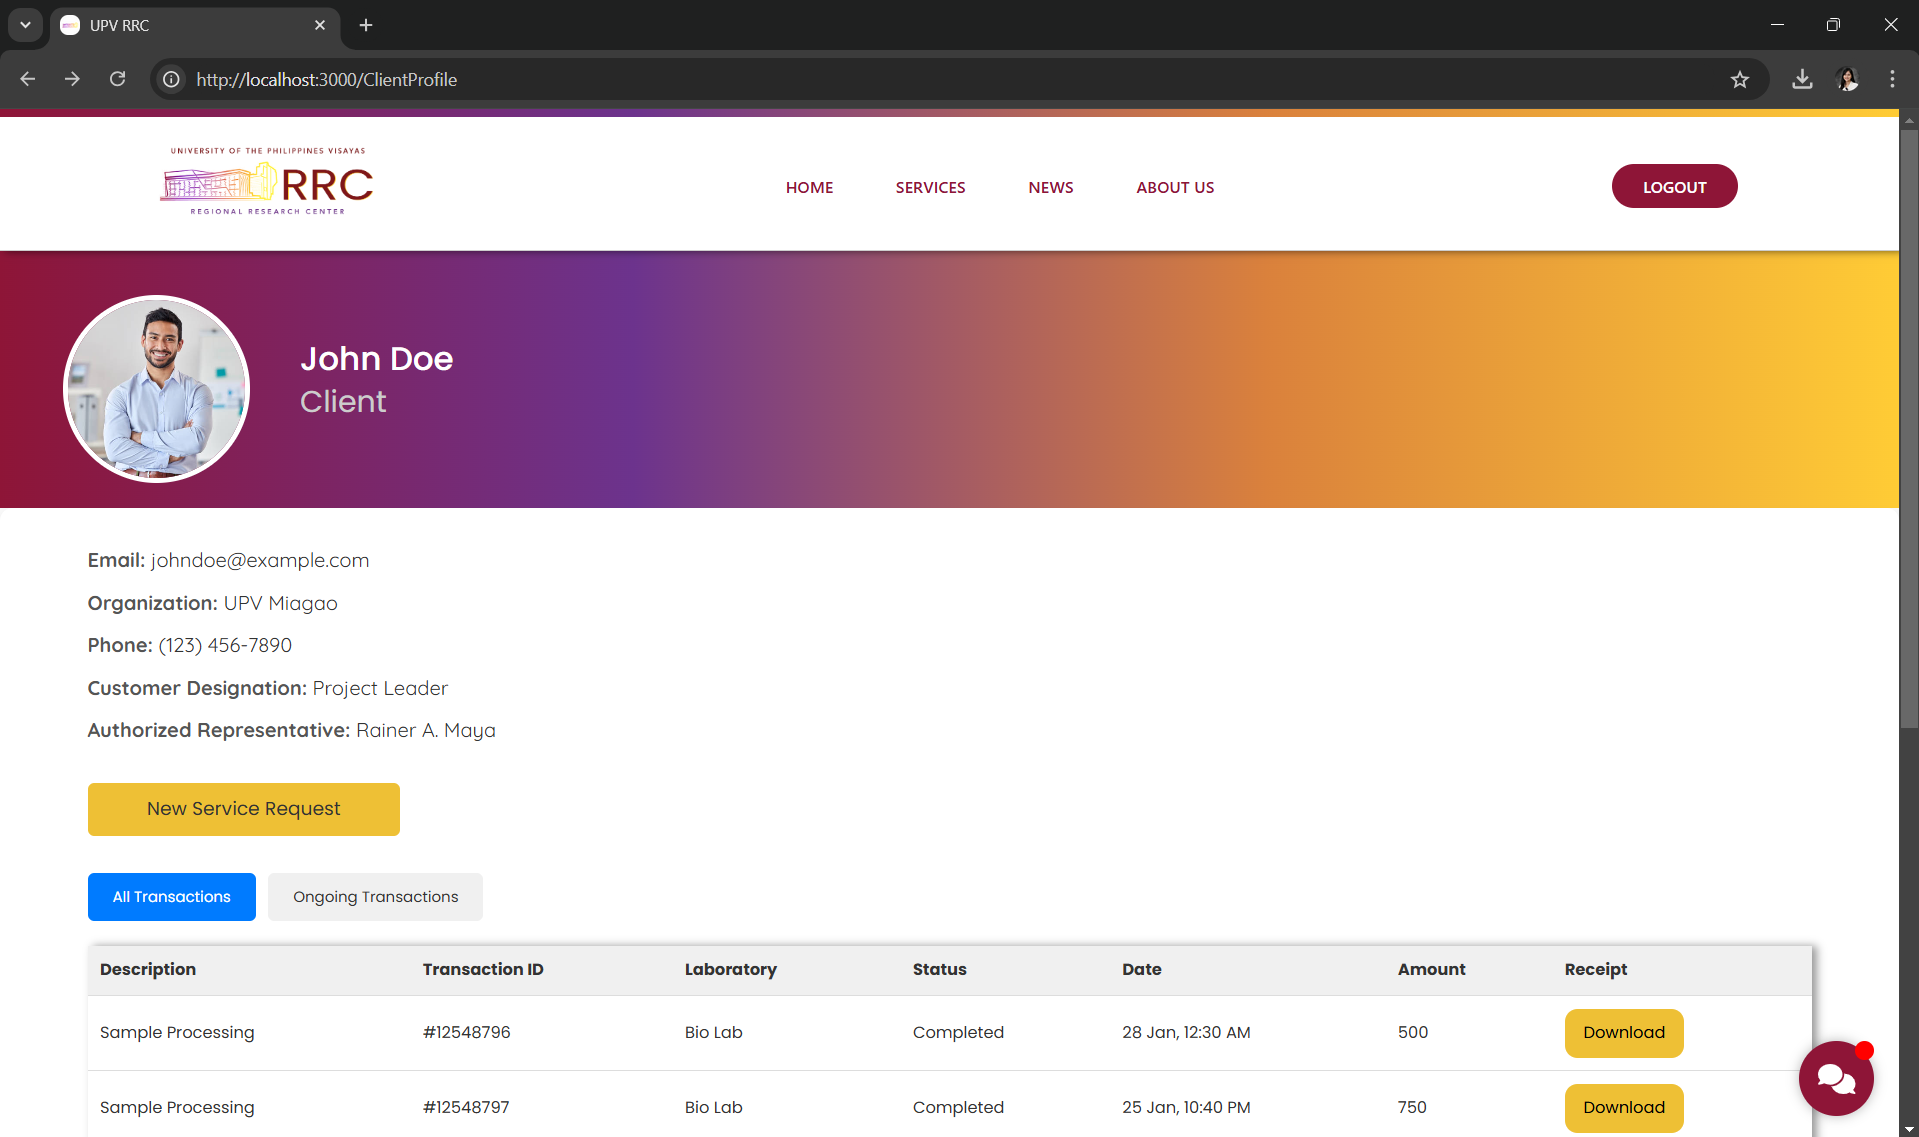
\includegraphics[width=0.8\textwidth]{client_dashboard.png}
	\caption{Client dashboard}
	\label{fig:client_dashboard}
\end{figure}

\newpage

\noindent \textbf{Services Page}

Figure \ref{fig:service_page} shows the service page. Each service has a separate page that includes a description of the service, pricing information, and instructions on how to avail the service. This structure facilitates easier navigation and helps users find the information they need efficiently.

\begin{figure}[h]
	\centering
	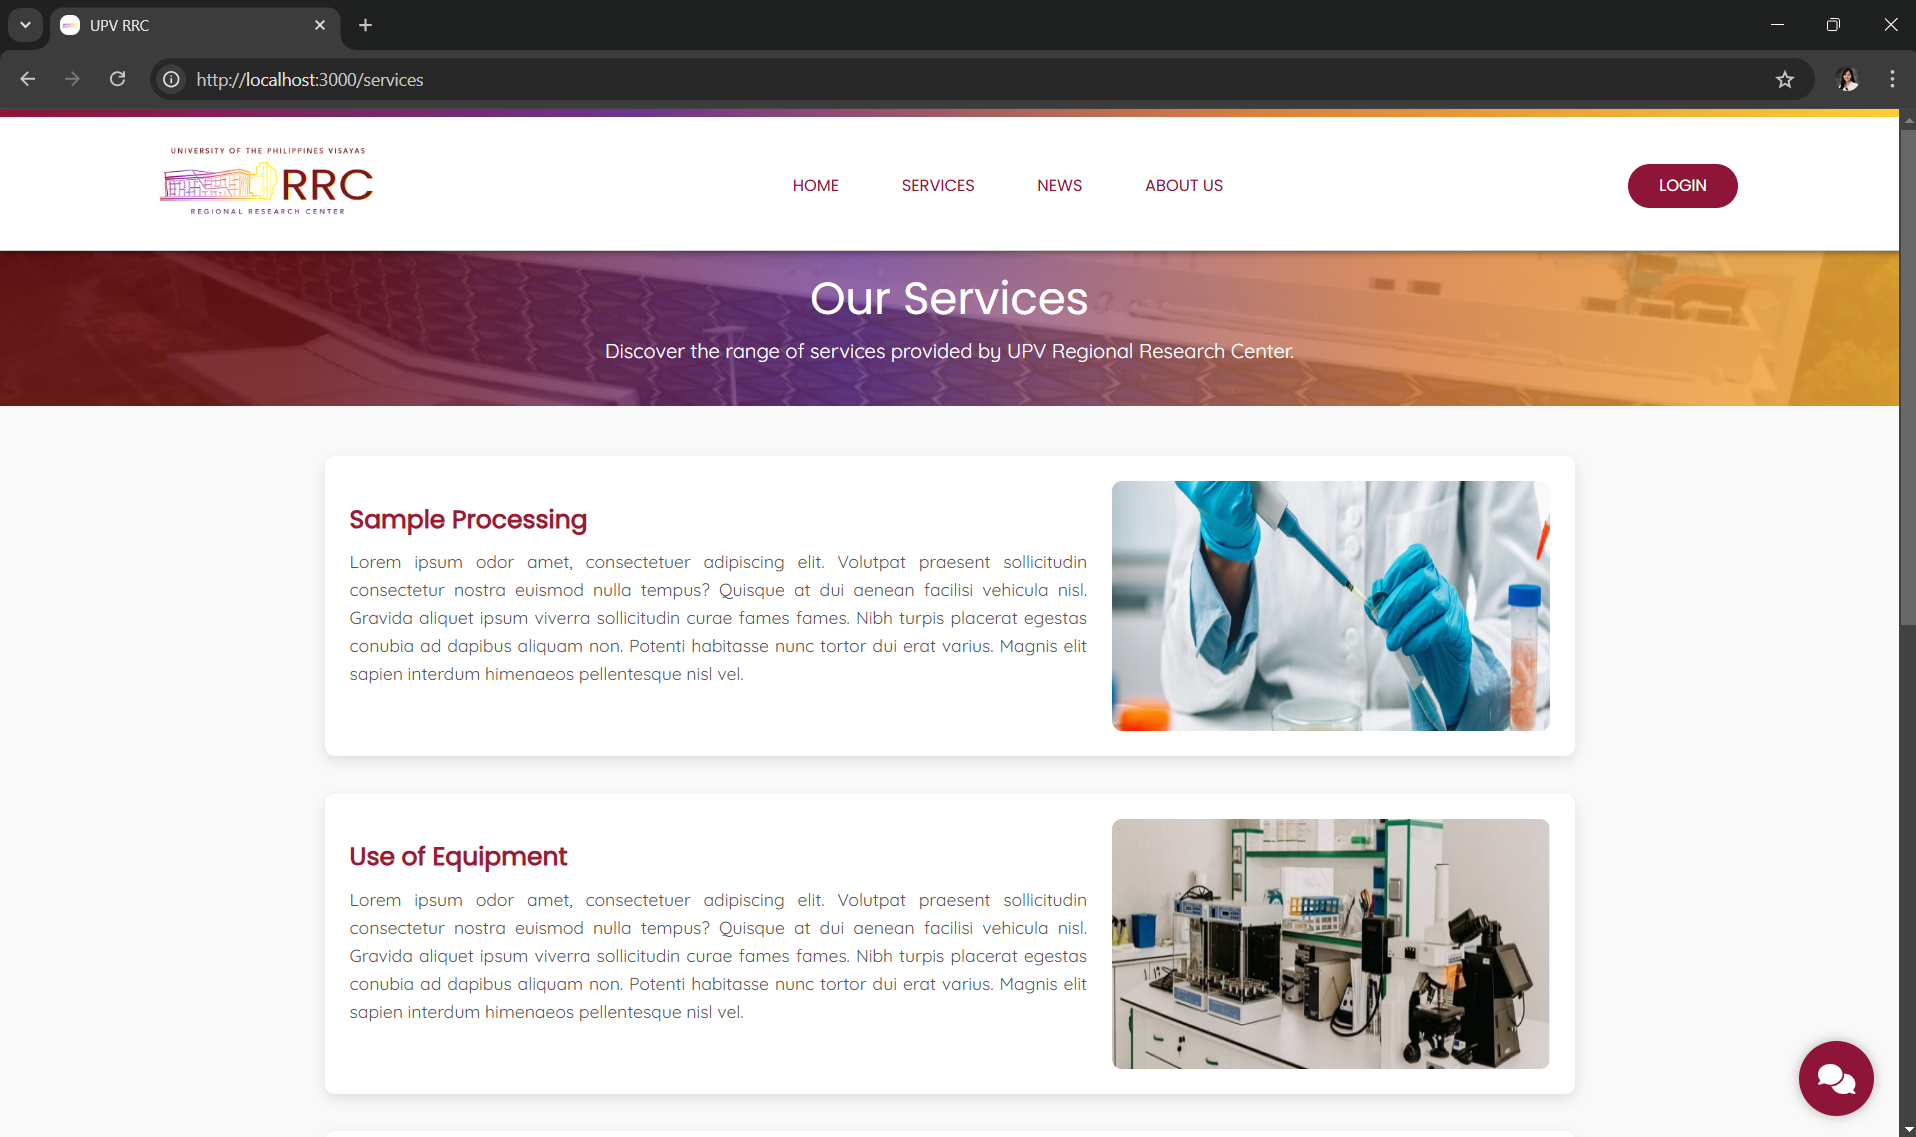
\includegraphics[width=0.8\textwidth]{service_page.png}
	\caption{Service Page}
	\label{fig:service_page}
\end{figure}



